% -*-latex-*-

\chapter{Physics Motivation}
\label{C4}

In previous chapters, we have discussed the unpolarized and polarized structure functions and their relations to the parton model. These structure functions have been extracted over a wide kinematic range during the past 40 years. However, data on the spin structure function $g_2$ at low energy is still lacking. Jefferson Lab Experiment E08-027 will provide precise data $g_2$ for the proton in the resonance region and extract the generalized longitudinal-transverse polarizability $\dlt$. $\dlt$ is expected to be a good test for the Chiral Perturbation Theory, as mentioned in \Cref{C3S1}. In addition, the $g_2$ data in the low $Q^2$ region could be used to provide a test of the Burkhardt-Cottingham (BC) sum rule. In this chapter, we will first give an overview of the previous experiments of the structure function measurement. The generalized longitudinal-transverse polarizability $\dlt$ and the BC sum rule will be discussed as the major motivation of experiment E08-027. The low $Q^2$ $g_2$ data will also help to improve the precision of the hyperfine structure calculation of hydrogen, which will also be discussed in this chapter.

\section{\texorpdfstring{Existing $g_2$ Data}{Existing g2 Data}}
\label{C4S1}

In \Cref{C2S2}, the relations between the spin structure functions and the cross-sections have been give as \cref{C2S2E25,C2S2E26}. To extract the spin structure function $g_1$ and $g_2$, one natural way is to measure the cross-section differences, which are defined as:
\begin{align} \label{C4S1E1}
\Delta\sigma_{\parallel} & = \dd{\sigma}^{\buildrel\rightarrow\over\Leftarrow}-\dd{\sigma}^{\buildrel\rightarrow\over\Rightarrow}, \\ \label{C4S1E2}
\Delta\sigma_{\perp} & = \dd{\sigma}^{\rightarrow\Uparrow}-\dd{\sigma}^{\rightarrow\Downarrow},
\end{align}
here the arrows indicate the polarization of the electrons and the target, $\buildrel\rightarrow\over\Leftarrow$ and $\buildrel\rightarrow\over\Rightarrow$ means the target is longitudinal polarized, $\rightarrow\Uparrow$ and $\rightarrow\Downarrow$ means the target is transversely polarized. However, the asymmetries are more commonly used in the scattering experiments to reduce the systematic uncertainty. The longitudinal asymmetry $A_{\parallel}$ and transverse asymmetry $A_{\perp}$ can be defined straightforwardly:
\begin{align} \label{C4S1E3}
A_{\parallel} & = \frac{\dd{\sigma}^{\buildrel\rightarrow\over\Leftarrow}-\dd{\sigma}^{\buildrel\rightarrow\over\Rightarrow}}{\dd{\sigma}^{\buildrel\rightarrow\over\Leftarrow}+\dd{\sigma}^{\buildrel\rightarrow\over\Rightarrow}} = \frac{\Delta\sigma_{\parallel}}{2\dd{\sigma}_{\mathrm{unpol}}}, \\ \label{C4S1E4}
A_{\perp} & = \frac{\dd{\sigma}^{\rightarrow\Uparrow}-\dd{\sigma}^{\rightarrow\Downarrow}}{\dd{\sigma}^{\rightarrow\Uparrow}+\dd{\sigma}^{\rightarrow\Downarrow}} = \frac{\Delta\sigma_{\perp}}{2\dd{\sigma}_{\mathrm{unpol}}}.
\end{align}
From the photon-absorption cross-sections formulation discussed in \Cref{C2S4SS1}, we could define another two asymmetries via \cref{C2S4E6,C2S4E7,C2S4E8,C2S4E9}:
\begin{align} \label{C4S1E5}
A_1 & = \frac{\stt}{\sigma_{T}} = \frac{g_1-\gamma^2g_2}{F_1}, \\ \label{C4S1E6}
A_2 & = \frac{\slt}{\sigma_{T}} = \frac{\gamma(g_1+g_2)}{F_1},
\end{align}
where $\gamma=Q/\nu$.

One can measure the longitudinal and transverse cross-section differences $\sigma_\parallel$ and $\sigma_\perp$ to extract $g_2$. As an alternative way, it is also possible to measure the asymmetries $A_\parallel$, $A_\perp$ or $A_1$, $A_2$ and combine existed $F_1$ results to extract $g_2$.

SLAC represented the earliest results for $g_2$ structure function in the DIS region \cite{Anthony1996}. During the same time, the SMC group at CERN used deep inelastic muon-nucleon scattering to extract the $g_1$ and $g_2$ structure functions for a proton target \cite{Adams1997}. Since $g_2$ is relatively small, more statistics are always required to extract it than for the extraction of $g_1$. Thus, some of the experiments like the SLAC experiment E155x \cite{Anthony2003} focused on transversely polarized targets to get enough statistics and extract $g_2$ using existing $g_1$ or $A_1$ data. Most recent results came from Jefferson Lab, where several experiments have collected a large amount of data covering a wide $Q^2$ range with a high intensity polarized electron beam. These JLab measurements covered both DIS and resonance regions.

\begin{figure}[b!]
  \centering
  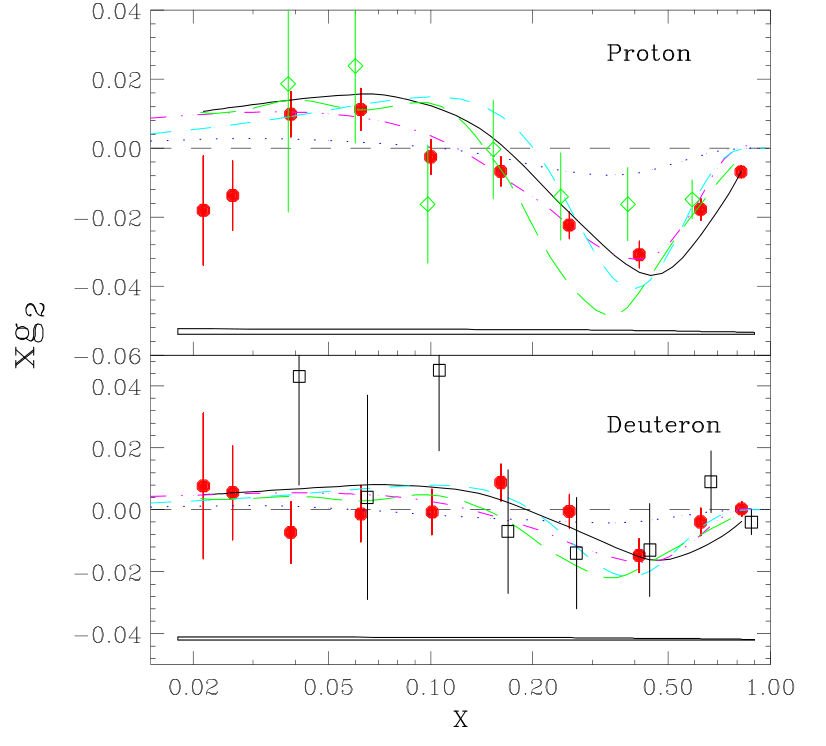
\includegraphics[width=0.75\textwidth]{figs/xg2p_E155x.png}
  \caption[$xg_2$ data from SLAC E155x, E143 and E155.]{$xg_2$ data from E155x (solid circle), E143 (open diamond) and E155 (open square). The $\gtww$ calculation result at the average $Q^2$ of E155x is also shown as the solid line as well as some model estimations from Stratmann \cite{Stratmann1993} (dash-dot), Song \cite{Song1996}(dot), Weigel and Gamberg \cite{Weigel2001} (short dash) and Wakamatsu \cite{Wakamatsu2000} (long dash). Plot reproduced from \cite{Anthony2003}. \label{C4S1F1}}
\end{figure}

The most precise DIS measurement results of $g_2$ for proton and deuteron targets were represented by SLAC experiment E155x \cite{Anthony2003}. The kinematic range was $0.02\leq x\leq 0.8$ and $0.7\leq Q^2 \leq 20$ GeV${}^2$. The SLAC experiments E143 \cite{Abe1998} and E155 \cite{Anthony2003} also contributed to the $g_2$ measurement of proton. The $g_2$ results from SLAC experiments E143, E155 and E155x are shown in \Cref{C4S1F1}. The solid curve in the figure represents the $\gtww$ calculation results using $g_1$ data. The curve shows that the the measurement and the leading twist estimation are consistent. However, the large error bars do not exclude the possible higher-twist effects.

As mentioned above, JLab also measured the $g_2$ structure function in the DIS region. The JLab experiment E97-103 measured $g_2$ for neutron and reported a two standard deviation difference from the leading twist expectation of $g_2^n$ \cite{Kramer2005}. The $Q^2$ coverage of this experiment is $0.58<Q^2<1.36$ GeV${}^2$ at $x\approx0.2$. \Cref{C4S1F2} shows the $xg_2^n$ results from JLab experiments E97-103, E99-117 \cite{Zheng2004} and SLAC experiment E155. The figure clearly represents the deviation between the experimental results and the leading twist estimation.

\begin{figure}[tb!]
  \centering
  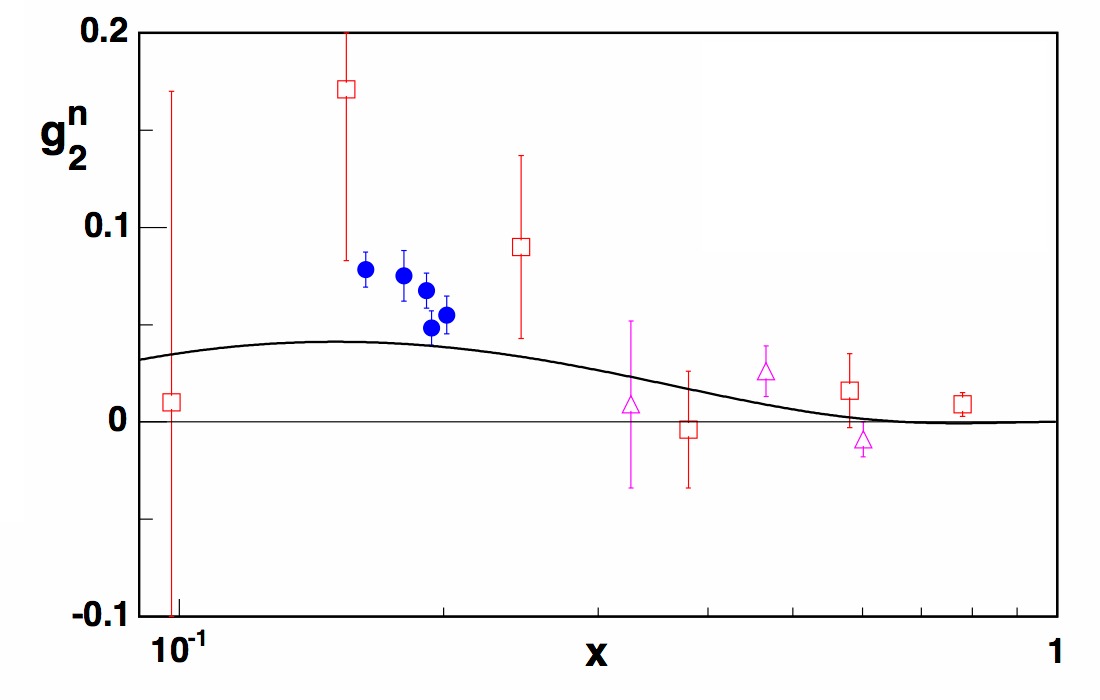
\includegraphics[width=0.6\textwidth]{figs/xg2n_E97103.png}
  \caption[$xg_2^n$ data from E97-103.]{$xg_2^n$ data from E97-103 (solid circle), E99-117 (open triangle) and E155 (open square). The solid curve shows $\gtww$ calculation at $Q^2=1.0$ GeV${}^2$. Plot reproduced from \cite{Kramer2005}. \label{C4S1F2}}
\end{figure}

From the discussion in \Cref{C3S1SS3}, we know that the quark-gluon interaction has stronger effect in the resonance region. The first experiment to measure $g_2$ in the resonance region was the SLAC experiment E143, at $Q^2=0.5$ GeV${}^2$ and 1.2 GeV${}^2$ \cite{Abe1998}. However the error bar is large for this measurement. JLab E94-010 collected a large amount of data to extract the neutron $g_2$ structure function at low $Q^2$ \cite{Amarian2004a}. The structure function $g_2$ was extracted from the longitudinal and transverse cross-section differences of a polarized ${}^3$He target. The results of ${}^3$He $g_2$ are shown in \Cref{C4S1F3}, which shows a significant deviation from the $\gtww$ estimation.

\begin{figure}[b!]
  \centering
  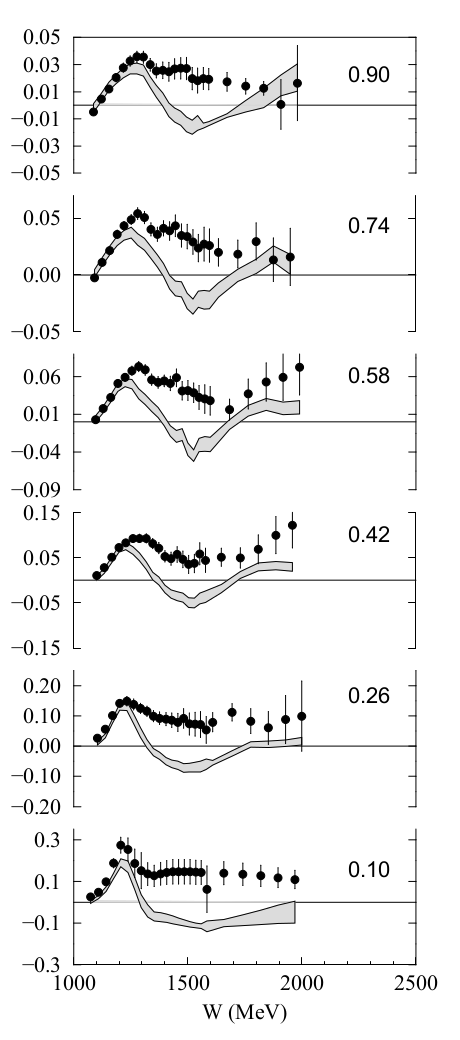
\includegraphics[width=0.55\textwidth]{figs/g2_E94010.png}
  \caption[${}^3$He $g_2$ data from E94-010.]{${}^3$He $g_2$ data from E94-010. The constant $Q^2$ values are indicated in GeV${}^2$ in each panel. The grey bands represent the $\gtww$ expectations at each corresponding $Q^2$ value. Plot reproduced from \cite{Amarian2004a}. \label{C4S1F3}}
\end{figure}

The Resonance Spin Structure (RSS) collaboration in JLab Hall B measured the proton $g_2$ structure function at $Q^2=1.3$ GeV${}^2$ \cite{Wesselmann2007}. Currently this is the lowest $Q^2$ measurement of $g_2^p$. The result is shown in \Cref{C4S1F4}. The leading twist behavior is clearly insufficient to describe the data.

\begin{figure}[tb!]
  \centering
  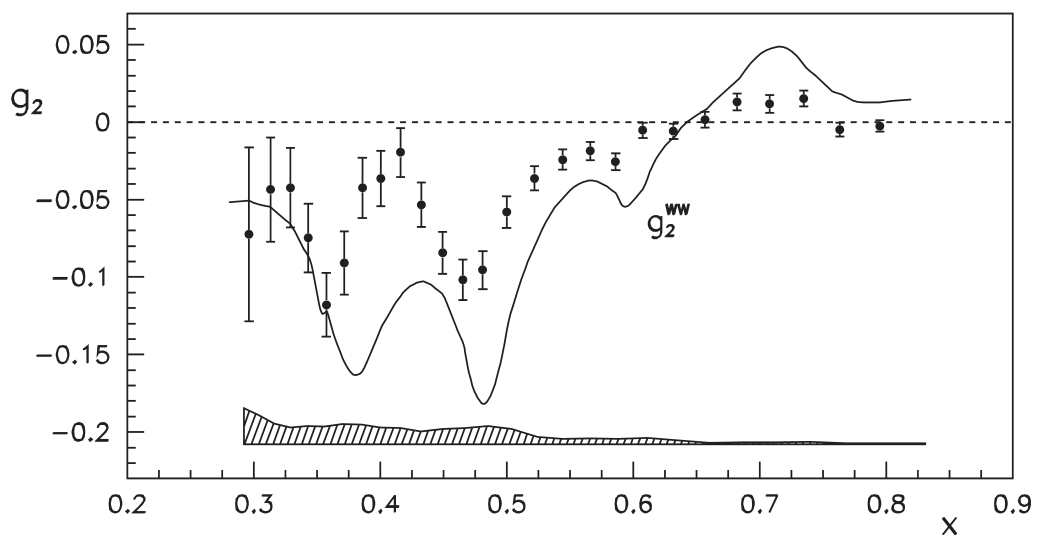
\includegraphics[width=0.75\textwidth]{figs/g2_RSS.png}
  \caption[Proton $g_2$ data from RSS experiment.]{Proton $g_2$ data from RSS experiment compared with the $\gtww$ expectations at $Q^2=1.3$ GeV${}^2$. Plot reproduced from \cite{Wesselmann2007}. \label{C4S1F4}}
\end{figure}

\section[Generalized Longitudinal-Transverse Polarizability]{Generalized Longitudinal-Transverse \\ Polarizability}
\label{C4S2}

\subsection{Sum Rules and Spin Polarizabilities}
\label{C4S2SS1}

In \Cref{C2S4SS2}, we discussed the formulation of real Compton scattering as well as the moments and sum rules which could be extracted from the dispersion relations of the forward real Compton scattering amplitude. Most of that discussions could be generalized for double virtual Compton scattering. In this case, the virtual photon has a third polarization component in addition to the $\epsilon_\pm$ defined in \cref{C2S4E13} due to the longitudinal degree of freedom. The longitudinal polarization vector could be defined as:
\begin{equation} \label{C4S2E1}
\epsilon_0 = \frac{1}{Q}(|\vec{q}|,0,0,q_0),
\end{equation}
where $q$ is the four-momentum of the virtual photon and we have chosen the $z$-axis in the direction of the photon propagation, i.e.,
\begin{equation} \label{C4S2E2}
q = (q_0,0,0,|\vec{q}|).
\end{equation}
All three polarization vectors and the momentum are orthogonal in the Lorentz metrics.

The forward real Compton scattering amplitude \cref{C2S4E17} could be generalized for the VVCS as \cite{Drechsel2003}:
\begin{equation} \label{C4S2E3}
\begin{split}
T(\nu,Q^2,\theta=0) = & \quad \vec{\epsilon}\,'^\star\cdot\vec{\epsilon}f_T(\nu,Q^2)+f_L(\nu,Q^2) \\
& +i\vec{\sigma}\cdot(\vec{\epsilon}\,'^\star\times\vec{\epsilon}\,)g_{TT}(\nu,Q^2)+i\vec{\sigma}\cdot[(\vec{\epsilon}\,'^\star-\vec{\epsilon}\,)\times\hat{q}]g_{LT}(\nu,Q^2).
\end{split}
\end{equation}
Notice the $f(\nu)$ and $g(\nu)$ has been generalized to $f_T(\nu,Q^2)$ and $g_{TT}(\nu,Q^2)$.

Similar to what we did in \Cref{C2S4SS2}, we can apply the optical theorem to \cref{C4S2E3} and get the relations between the four amplitudes and the four partial cross-sections of the inclusive scattering in \cref{C2S4E4}, which gives:
\begin{equation} \label{C4S2E4}
\begin{aligned}
& \Im f_T(\nu,Q^2) = \frac{K}{4\pi}\sigma_T(\nu,Q^2), & \qquad & \Im f_L(\nu,Q^2) = \frac{K}{4\pi}\sigma_L(\nu,Q^2), \\
& \Im g_{TT}(\nu,Q^2) = \frac{K}{4\pi}\stt(\nu,Q^2), & \qquad & \Im g_{LT}(\nu,Q^2) = \frac{K}{4\pi}\slt(\nu,Q^2),
\end{aligned}
\end{equation}
where $K$ is the virtual photon flux defined in \cref{C2S4E2} or \cref{C2S4E3}.

Considering the spin-dependent amplitude $g_{TT}$ and assuming it converges appropriately at high energy, there is an unsubtracted dispersion relation \cite{Drechsel2003}:
\begin{equation} \label{C4S2E5}
\Re[g_{TT}(\nu,Q^2)-g_{TT}^{\mathrm{pole}}(\nu,Q^2)] = \frac{\nu}{2\pi^2}\pv{\int_{\nu_0}^\infty\dd{\nu'}\frac{K(\nu',Q^2)\stt(\nu',Q^2)}{\nu'^2-\nu^2}},
\end{equation}
where $g_{TT}^{\mathrm{pole}}$ is the elastic contribution. The lower limit of the integration $\nu_0$ is the pion-production threshold. As what we did for real Compton scattering, we could also perform a low energy expansion for the non-pole contribution of $g_{TT}$ similar to \cref{C2S4E20}:
\begin{equation} \label{C4S2E6}
\Re[g_{TT}(\nu,Q^2)-g_{TT}^{\mathrm{pole}}(\nu,Q^2)] = \frac{2\alpha}{M^2}I_A(Q^2)\nu+\gamma_0(Q^2)\nu^3+\order{\nu^5}.
\end{equation}

Comparing \cref{C4S2E6} and the Taylor expansion of \cref{C4S2E5}, the $\order{\nu}$ term yields a generalized GDH sum rule \cite{Drechsel2001}:
\begin{equation} \label{C4S2E7}
\begin{split}
I_A(Q^2) & = \frac{M^2}{4\pi^2\alpha}\int_{\nu_0}^\infty\dd{\nu}\frac{K(\nu,Q^2)}{\nu}\frac{\stt(\nu,Q^2)}{\nu}, \\
& = \frac{2M^2}{Q^2}\int_0^{x_0}\dd{x}\left\{g_1(x,Q^2)-\frac{4M^2}{Q^2}x^2g_2(x,Q^2)\right\}.
\end{split}
\end{equation}
The $\order{\nu^3}$ term leads to a generalized form of the forward spin polarizability $\gamma_0$:
\begin{equation} \label{C4S2E8}
\begin{split}
\gamma_0(Q^2) & = \frac{1}{2\pi^2}\int_{\nu_0}^\infty\dd{\nu}\frac{K(\nu,Q^2)}{\nu}\frac{\stt(\nu,Q^2)}{\nu^3}, \\
& = \frac{16\alpha M^2}{Q^6}\int_0^{x_0}\dd{x}x^2\left\{g_1(x,Q^2)-\frac{4M^2}{Q^2}x^2g_2(x,Q^2)\right\}.
\end{split}
\end{equation}
The term proportional to $g_2$ can be dropped when $Q^2$ is large.

For amplitude $g_{LT}$, we have an unsubtracted dispersion relation in the form of \cite{Drechsel2003}:
\begin{equation} \label{C4S2E9}
\Re[g_{LT}(\nu,Q^2)-g_{LT}^{\mathrm{pole}}(\nu,Q^2)] = \frac{1}{2\pi^2}\pv{\int_{\nu_0}^\infty\dd{\nu'}\frac{\nu'K(\nu',Q^2)\slt(\nu',Q^2)}{\nu'^2-\nu^2}}.
\end{equation}
The low energy expansion of the non-pole contribution of $g_{LT}$ gives:
\begin{equation} \label{C4S2E10}
\Re[g_{LT}(\nu,Q^2)-g_{LT}^{\mathrm{pole}}(\nu,Q^2)] = \frac{2\alpha}{M^2}QI_3(Q^2)\nu+Q\dlt(Q^2)\nu^2+\order{\nu^4},
\end{equation}
where the leading term is a sum rule for $I_3(Q^2)$:
\begin{equation} \label{C4S2E11}
\begin{split}
I_3(Q^2) & = \frac{M^2}{4\pi^2\alpha}\int_{\nu_0}^\infty\dd{\nu}\frac{K(\nu,Q^2)}{\nu}\frac{\slt(\nu,Q^2)}{Q}, \\
& = \frac{2M^2}{Q^2}\int_0^{x_0}\dd{x}\left\{g_1(x,Q^2)+g_2(x,Q^2)\right\},
\end{split}
\end{equation}
and the $\order{\nu^2}$ gives the generalized longitudinal-transverse polarizability:
\begin{equation} \label{C4S2E12}
\begin{split}
\dlt(Q^2) & = \frac{1}{2\pi^2}\int_{\nu_0}^\infty\dd{\nu}\frac{K(\nu,Q^2)}{\nu}\frac{\slt(\nu,Q^2)}{Q\nu^2}, \\
& = \frac{16\alpha M^2}{Q^6}\int_0^{x_0}\dd{x}x^2\left\{g_1(x,Q^2)+g_2(x,Q^2)\right\}.
\end{split}
\end{equation}

The forward VVCS amplitude $T(\nu,Q^2,\theta=0)$ can also be written in the form of an one-to-one correspondence with the structure functions \cite{Drechsel2003}:
\begin{equation} \label{C4S2E13}
\begin{split}
T(\nu,Q^2,\theta=0) = \epsilon_\mu'^{\star}\epsilon_\nu & \left\{\left(\frac{q^\mu q^\nu}{q^2}-g^{\mu\nu}\right)T_1(\nu,Q^2)\right. \\
& +\frac{1}{P\cdot q}(P^\mu-\frac{P\cdot q}{q^2}q^\mu)(P^\nu-\frac{P\cdot q}{q^2}q^\nu)T_2(\nu,Q^2) \\
& +i\varepsilon^{\mu\nu\alpha\beta}\frac{1}{M}q_\alpha S_\beta S_1(\nu,Q^2) \\
& \left.+i\varepsilon^{\mu\nu\alpha\beta}\frac{1}{M^3}q_\alpha(P\cdot qS_\beta-S\cdot qP_\beta)S_2(\nu,Q^2)\right\},
\end{split}
\end{equation}
where $P^\mu$ and $S^\mu$ are the four momentum and the spin vector of the nucleon and $T_1$, $T_2$, $S_1$, $S_2$ are four VVCS amplitudes which is covariant under Lorentz transform.

Since we only discussed te spin-flip amplitudes $g_{TT}$ and $g_{LT}$ in this section, we will focus on $S_1$ and $S_2$, which can be expressed as a linear combination of $g_{TT}$ and $g_{LT}$:
\begin{equation} \label{C4S2E14}
\begin{split}
S_1(\nu,Q^2) & = \frac{\nu M}{\nu^2+Q^2}\left(g_{TT}(\nu,Q^2)+\frac{Q}{\nu}g_{LT}(\nu,Q^2)\right), \\
S_2(\nu,Q^2) & = -\frac{M^2}{\nu^2+Q^2}\left(g_{TT}(\nu,Q^2)-\frac{\nu}{Q}g_{LT}(\nu,Q^2)\right).
\end{split}
\end{equation}
We can construct unsubtracted dispersion relations for $S_1$ and $S_2$ with a similar procedure as $g_{LT}$ and $g_{TT}$.

For amplitude $S_1$, the low energy expansion has the form:
\begin{multline} \label{C4S2E15}
\Re[S_1(\nu,Q^2)-S_1^{\mathrm{pole}}(\nu,Q^2)] = \\
\frac{2\alpha}{M^2}I_1(Q^2)+\left[\frac{2\alpha}{MQ^2}(I_A(Q^2)-I_1(Q^2))+M\dlt(Q^2)\right]\nu^2+\order{\nu^4},
\end{multline}
where the leading term leads to a sum rule:
\begin{equation} \label{C4S2E16}
\begin{split}
I_1(Q^2) & \equiv \frac{2M^2}{Q^2}\int_0^{x_0}\dd{x}g_1(x,Q^2) \\
& = \frac{M^2}{4\pi^2\alpha}\int_{\nu_0}^\infty\dd{\nu}\frac{K(\nu,Q^2)}{\nu^2+Q^2}\left\{\stt(\nu,Q^2)+\frac{Q}{\nu}\slt(\nu,Q^2)\right\},
\end{split}
\end{equation}
which reduces to the GDH sum rule at $Q^2=0$ (real photon limit). $I_1(Q^2)$ has a limit at large $Q^2$:
\begin{equation} \label{C4S2E17}
I_1(Q^2)\rightarrow(2M^2/Q^2)\Gamma_1(Q^2), \qquad Q^2\rightarrow\infty,
\end{equation}
where
\begin{equation} \label{C4S2E18}
\Gamma_1(Q^2) \equiv \int_0^1\dd{x}g_1(x,Q^2).
\end{equation}
Here the $\Gamma_1$ is the first moment of structure function $g_1$. The Bjorken sum rule \cite{Bjorken1966,Bjorken1970} gives a prediction of the isovector combination $\Gamma_1^p-\Gamma_1^n$ with the QCD radiative corrections \cite{Larin1991}:
\begin{multline} \label{C4S2E19}
\Gamma_1^p-\Gamma_1^n = \frac{1}{6}g_A \\
\times\left\{1-\left(\frac{\alpha_S(Q^2)}{\pi}\right)-3.5833\left(\frac{\alpha_S(Q^2)}{\pi}\right)^2-20.2153\left(\frac{\alpha_S(Q^2)}{\pi}\right)^3+\cdots\right\},
\end{multline}
where $g_A$ is the axial-vector coupling constant. At $Q^2=5$ GeV${}^2$, \cref{C4S2E19} gives $\Gamma_1^p-\Gamma_1^n=0.182\pm0.005$ if only the three light quark flavors are considered. The next-to-leading order fit to global $g_1$ data gives $\Gamma_1^p-\Gamma_1^n=0.176\pm0.003\pm0.007$ \cite{Anthony2000}, in agreement with the theoretical calculation.

The unsubtracted dispersion relations of the amplitude $S_2$ lead to the Burkhardt-Cottingham sum rule. Assume the high energy behavior of this amplitude is given by $S_2\rightarrow\nu^{\alpha_2}$ with $\alpha_2<-1$ when $\nu\rightarrow\infty$, there should be a dispersion relation for $\nu S_2$. By subtracting the dispersion relation of $\nu S_2$ from the dispersion relation of $S_2$ multiplied by $\nu$, we could get a ``super-convergence relation'' \cite{Burkhardt1970}:
\begin{equation} \label{C4S2E20}
\int_0^1\dd{x}g_2(x,Q^2) = 0.
\end{equation}
This indicates that the elastic and the inelastic contributions to the first moment of $g_2$ should cancel for any value of $Q^2$. The elastic and inelastic contributions to the integral can be separated, thus the BC sum rule can be expressed as:
\begin{equation} \label{C4S2E21}
I_2(Q^2) \equiv \frac{2M^2}{Q^2}\int_0^{x_0}\dd{x}g_2(x,Q^2) = \frac{1}{4}F_P(Q^2)(F_D(Q^2)+F_P(Q^2)),
\end{equation}
where $F_P$ is the Pauli form factor and $F_D$ is the Dirac form factor. The integral $I_2$ can also be written in terms of the photon-absorption cross-sections and the Sachs form factor $G_E$ and $G_M$:
\begin{equation} \label{C4S2E22}
\begin{split}
I_2(Q^2) & = \frac{M^2}{4\pi^2\alpha}\int_{\nu_0}^\infty\frac{K(\nu,Q^2)}{\nu^2+Q^2}\left\{-\stt(\nu,Q^2)+\frac{\nu}{Q}\slt(\nu,Q^2)\right\} \\
& = \frac{1}{4}\frac{G_M(Q^2)(G_M(Q^2)-G_E(Q^2))}{1+\tau},
\end{split}
\end{equation}
with $\tau=Q^2/4M^2$.

\subsection{Existing World Data for Spin Polarizabilities}
\label{C4S2SS2}

From the discussion in \Cref{C2S4SS2}, we know that the nucleon polarizabilities are fundamental observables that characterize nucleon structure. The electric and magnetic polarizabilities $\alpha$ and $\beta$ describe the response of a nucleon to an external electromagnetic field. Real photon Compton scattering experiments were performed to measure these two quantities since they are related to the spin non-flip forward Compton scattering amplitude \cite{Olmos2001,Tonnison1998}. The forward spin polarizability $\gamma_0$ is associated with the spin flip amplitude. It has been measured at MAMI (Mainz) with a circularly polarized photon beam on a longitudinally polarized proton target \cite{Ahrens2001}.

In the previous section, we have discussed that these polarizabilities could be generalized in VVCS. The generalized polarizabilities defined in \cref{C4S2E8,C4S2E12} have an extra $1/\nu^2$ weighting in the integrand compared to the corresponding leading moments. Thus, the contribution of the large-$\nu$ region to these integrals are suppressed by this weight. With this suppression effect, the generalized spin polarizabilities become a perfect tool to probe the nucleon structure in the chiral perturbation region. The generalized polarizabilities have been evaluated with next-to-leading order (NLO) $\chi$PT calculations at low $Q^2$ \cite{Bernard2003,Kao2003}. As mentioned in \Cref{C3S1SS3}, the nucleon resonances, especially the $\Delta$ resonance, play an important role in the $\chi$PT calculations. Ref. \cite{Bernard2003} and \cite{Kao2003} have pointed out that the generalized longitudinal polarizability $\dlt$ is insensitive to the $\Delta$ resonance compare with the generalized forward spin polarizability $\gamma_0$. The effects from the $\Delta$ resonance contribution are expected to be important in $\gamma_0$ but are supposed to largely cancel in $\dlt$.

\begin{figure}[tb!]
  \centering
  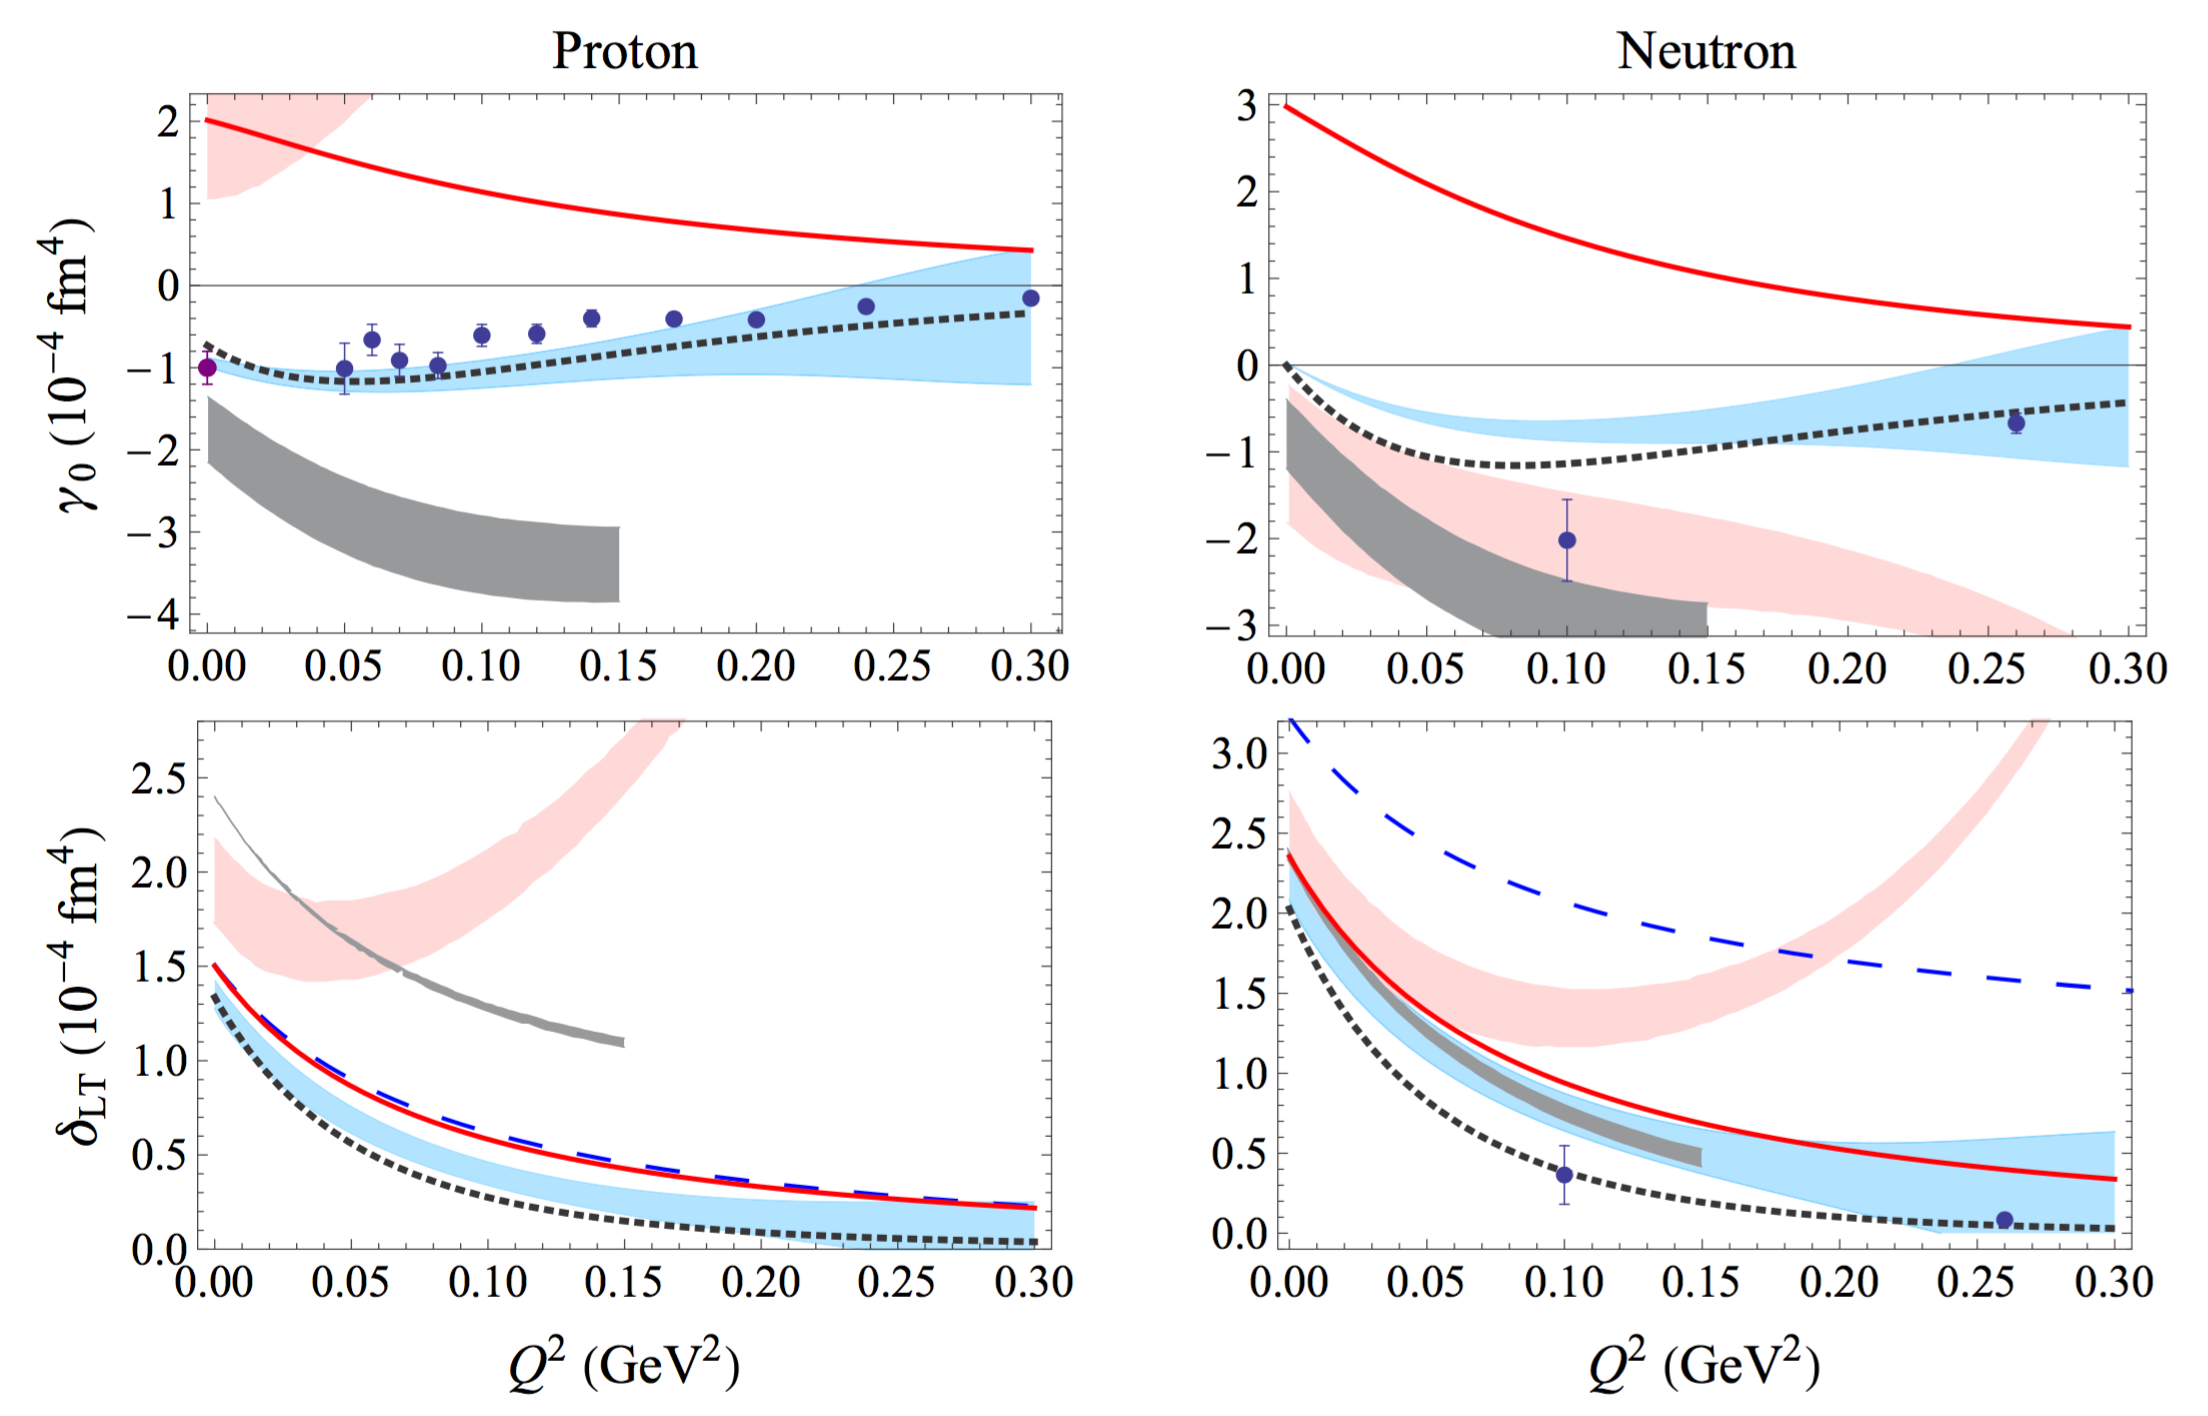
\includegraphics[width=\textwidth]{figs/g0_dlt_xpt.png}
  \caption[Generalized spin polarizability $\gamma_0$ and $\dlt$ of proton and neutron.]{Generalized spin polarizability $\gamma_0$ and $\dlt$ of proton and neutron. The neutron data are from E94-010 experiment \cite{Amarian2004b}. The proton data at $Q^2=0$ (purple dot) are from ELSA \cite{Dutz2003}, and at finite $Q^2$ (blue dots) from EG1 experiment at JLab \cite{Prok2009}. The blue dashed line is the HB$\chi$PT calculation \cite{Kao2003}, off the scale in the upper panels. The red bands shows the IR version of RB$\chi$PT calculation \cite{Bernard2003}. The grey bands are the first RB$\chi$PT calculation from Ref. \cite{Bernard2013}. The red solid lines and blue bands shows the most recent LO and NLO RB$\chi$PT calculations respectively \cite{Lensky2014}. Black dotted lines represents the empirical evaluation using the Mainz online partial-wave analysis of meson electroproduction (MAID). Plot reproduced from \cite{Lensky2014}. \label{C4S2F1}}
\end{figure}

The experimental results compared with the $\chi$PT calculations are shown in \Cref{C4S2F1}. The first results of neutron $\gamma_0(Q^2)$ and $\dlt(Q^2)$ were obtained from JLab Hall A experiment E94-010 \cite{Amarian2004b} (blue dots in the neutron panels). The data are compared with a HB$\chi$PT calculation \cite{Kao2003} (blue dashed line) and an infrared-regularized (IR) version of RB$\chi$PT calculation \cite{Bernard2003} (red bands) which is relativisitic but has an unphysical analytic structure. At the lowest $Q^2$ point, the IR version of RB$\chi$PT calculation of $\gamma_0$ including the resonance contributions agrees with the experimental result from E94-010 for neutron. But there are discrepancies between the HB$\chi$PT calculation of $\gamma_0$ and the experimental result even at the lowest $Q^2$ point. For $\dlt$, both the HB$\chi$PT calculation and the IR version of RB$\chi$PT calculation indicates a significant disagreement with the data, which is known as the ``$\dlt$ puzzle''. Since the $\dlt$ is insensitive to the $\Delta$ resonance contribution, it is believed that $\dlt$ is a more suitable testing base for the $\chi$PT compare with $\gamma_0$. A first RB$\chi$PT calculation (with no unphysical analytical structure) from Ref. \cite{Bernard2013} shows that it agrees much better than the HB$\chi$PT and the IR version of the RB$\chi$PT for $\gamma_0$ (grey bands). The most recent calculation from Ref. \cite{Lensky2014} using LO and NLO RB$\chi$PT shows that the $\dlt$ data agrees with their NLO calculation (blue bands). The neutron $\gamma_0$ and $\dlt$ data in \Cref{C4S2F1} is obtained from the JLab experiment E94-010. The proton $\dlt$ data is required to complete the comparison. This is one of the major physics motivation of the JLab experiment E08-027.

\section{Burkhardt-Cottingham Sum Rule}
\label{C4S3}

In \Cref{C4S2SS1}, we have discussed the dispersion relations for the covariant spin-dependent VVCS amplitudes $S_2$. The dispersion relations for $S_2$ and $\nu S_2$ lead to a sum rule for $g_2$ which is valid for all $Q^2$ \cite{Burkhardt1970}:
\begin{equation} \label{C4S3E1}
\Gamma_2(Q^2) = \int_0^1\dd{x}g_2(x,Q^2) = 0.
\end{equation}
The existence of the dispersion relation of $\nu S_2$ requires $S_2\rightarrow\nu^{\alpha_2}$ with $\alpha_2<-1$ when $\nu\rightarrow\infty$. Thus, the convergence condition of the integral leads to $g_2(x,Q^2)\rightarrow x^{\tilde{\alpha}_2}$ with $\tilde{\alpha}_2>-1$ when $x\rightarrow0$, which means that $g_2$ must exhibit Regge behavior at low $x$ and does not exhibit a delta function singularity at $x=0$ \cite{Jaffe1991}.

The first measurement of the moment $\Gamma_2$ is the SLAC experiment E155, which included the result of proton, deuteron and neutron. JLab Hall A has collected a large amount of data to extract the BC integral of neutron over a wide kinematic range in several experiments: E94-010 \cite{Amarian2004a}, E97-110 and E01-012. Since it is impossible to cover the full integral range, the full ($0<x<1$) integral is evaluated using the elastics form factors for the elastic contribution, and assuming $g_2=\gtww$ in the very low-$x$ region. The full integral exhibits a significant cancellation of the inelastic (resonance and DIS) and elastic contributions. The neutron data agrees with the BC sum rule prediction within uncertainty.

\begin{figure}[tb!]
  \centering
  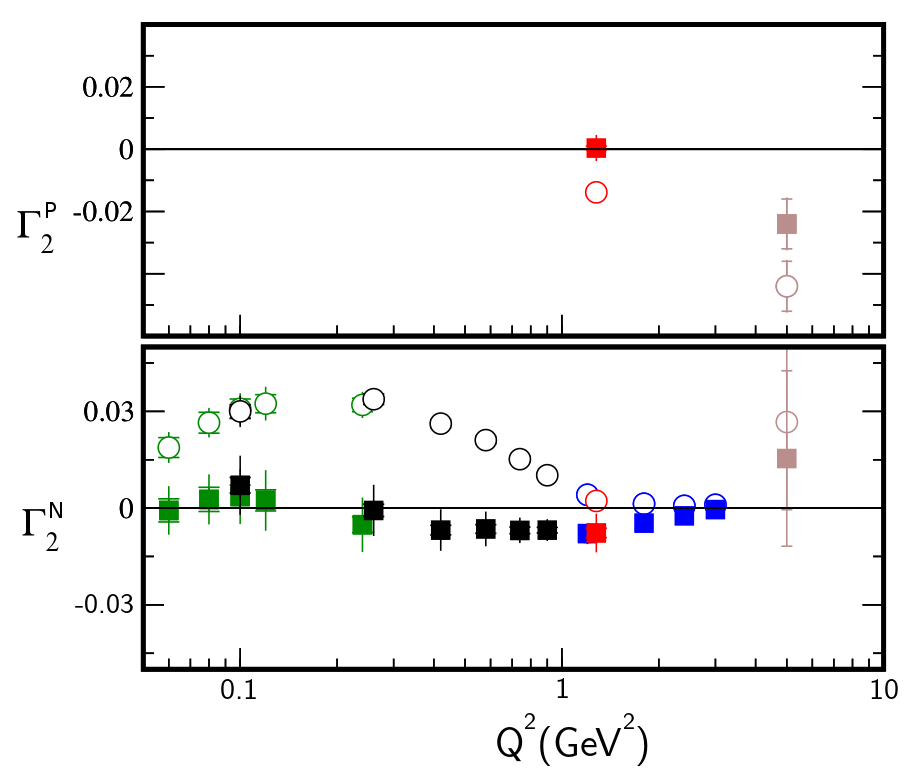
\includegraphics[width=0.75\textwidth]{figs/BC_all.png}
  \caption[The verification of the BC sum rule.]{The verification of the BC sum rule from JLab Hall C experiment RSS (red) and Hall A experiments E94-010 \cite{Amarian2004a} (black), E97-110 (green) and E01-012 (blue), together with SLAC experiment E155x \cite{Anthony2003} (brown). The open circles are the measured values and the solid squares are the total moments including the elastic and estimated contributions from high energy region. The data from experiments RSS and E97-110 are still preliminary. Plot reproduced from \cite{Chen2010}. \label{C4S3F1}}
\end{figure}

On the other hand, the proton BC integral deviated from zero by three standard deviations in SLAC experiment E155x \cite{Abe1998}. E155x covered the $x$ range from 0.02 to 0.8 and its $Q^2$ coverage $0.8-8.2$ GeV${}^2$ was averaged to 5 GeV${}^2$. JLab experiment RSS also measured the BC integral for proton which covered $W<1.910$ MeV at $Q^2\approx1.3$ GeV${}^2$. The preliminary result agrees with the BC sum rule prediction within the experimental error. The experimental results for verification of the BC sum rule are summarized in \Cref{C4S3F1}.

\section{Proton Hyperfine Structure}
\label{C4S4}

The hydrogen hyperfine splitting has been measured to a relative accuracy of $10^{-13}$ according to the discussion in Ref. \cite{Nazaryan2006}:
\begin{equation} \label{C4S4E1}
\Delta E = 1420.405 751 766 7(9) \text{MHz}.
\end{equation}
This value could be calculate in QED. $\Delta E$ can be expressed in terms of the so-called Fermi energy $E_F$ which is the leading order contribution to the ground state hyperfine splitting as $\Delta E = (1+\delta)E_F$, where the correction $\delta$ is given by:
\begin{equation} \label{C4S4E2}
\delta = 1+(\delta_{\mathrm{QED}}+\delta_R+\delta_{\mathrm{small}})+\Delta_S.
\end{equation}
Here the $\delta_{\mathrm{QED}}$ represents the QED radiative correction which has been calculated to very high accuracy. The $\delta_R$ accounts the recoil effects and the $\delta_{\mathrm{small}}$ term contains all other small corrections such as the weak interaction correction.

The $\Delta_S$ term in \cref{C4S4E2} represents the proton structure correction has the largest uncertainty. $\Delta_S$ is conventionally split into two terms:
\begin{equation} \label{C4S4E3}
\Delta_S = \Delta_Z+\Delta_{\mathrm{pol}},
\end{equation}
where $\Delta_Z$ can be determined from elastic scattering \cite{GEP} and $\Delta_{\mathrm{pol}}$ contains the contributions from excited proton \cite{Iddings1965,Faustov2002}:
\begin{equation} \label{C4S4E4}
\Delta_{\text{pol}} = \frac{\alpha m_e}{\pi g_pm_p}(\Delta_1+\Delta_2),
\end{equation}
where $\Delta_1$ involves the Pauli form factor and the $g_1$ structure function, and $\Delta_2$ only depends on the $g_2$ structure function:
\begin{equation} \label{C4S4E5}
\Delta_2 = -24m_p^2\int_0^{\infty}\frac{\dd{Q}^2}{Q^4}B_2(Q^2),
\end{equation}
where
\begin{equation} \label{C4S4E6}
B_2(Q^2) = \int_0^{x_{\mathrm{th}}}\dd{x}\beta_2(\tau)g_2(x,Q^2).
\end{equation}
and
\begin{equation} \label{C4S4E7}
\beta_2(\tau) = 1+2\tau-2\sqrt{\tau(\tau+1)},
\end{equation}
with $\tau=\nu^2/Q^2$ and $x_{\mathrm{th}}$ is the pion production threshold.

$\Delta_1$ could be determined with data but to evaluate $\Delta_2$ physicists still heavily rely on models since proton $g_2$ data are still lacking. The $Q^2$ weighting in \cref{C4S4E5} indicates that $\Delta_2$ is dominated by the contribution at low $Q^2$ \cite{Nazaryan2006}. Thus, precision data of proton $g_2$ at low $Q^2$ is needed to evaluate $\Delta_2$.

%%%%%%%%%%%%%%%%%%%%%%%%%%%%%%%%%%%%%%%%%%%%%%%%%%%%%%%%%%%%%%%%%%%%%%
% -*-latex-*-
